% This file demonstrates how to use the IEEEConf LaTeX2e macro package,
% to prepare a manuscript for proceedings on CD of the conference
% FedCSIS
%
\documentclass[a4paper,10pt]{IEEEtran}
%\documentclass[a4paper]{IEEEconf}



% Usepackages
\usepackage{cite}
% provides various features to facilitate writing math formulas and to improve the typographical quality of their output.
\usepackage{amsmath}
% \usepackage[cmex10]{amsmath}
\interdisplaylinepenalty=2500
\usepackage{amssymb,amsfonts}
\usepackage{algorithmic}
\usepackage{graphicx}
% \usepackage{graphicx}
\usepackage{textcomp}
\usepackage{xcolor}

% formatting from IEEE conference. Needs to be fitted with our natbib
\def\BibTeX{{\rm B\kern-.05em{\sc i\kern-.025em b}\kern-.08em
		T\kern-.1667em\lower.7ex\hbox{E}\kern-.125emX}}

%%%%%%%%%%%%%%%%%%%%%%%%
%Article stuff
%%%%%%%%%%%%%%%%%%%%%%%%
% This package serves to balance the column lengths on the last page of the document.
% please, insert \balance command in the left column of the last page
\usepackage{balance}
\usepackage{supertabular}
\usepackage{paralist}
\usepackage{booktabs}

%% to enable \thank command
\IEEEoverridecommandlockouts 
% to typeset algorithms
\usepackage{algorithm}
%\usepackage{algpseudocode}
% to typeset code fragments
\usepackage{listings}
% to make an accent \k be available
\usepackage[T1]{fontenc}
% por urls typesetting and breaking
\usepackage{url}
% for vertical merging table cells
\usepackage{multirow}
\usepackage{siunitx}


%%%%%%%%%%%%%%%%%%%%%%%%
%Mixed packages
%%%%%%%%%%%%%%%%%%%%%%%%
\usepackage[hidelinks]{hyperref}
\usepackage{graphicx}
\usepackage[textsize=scriptsize]{todonotes}
\usepackage{glossaries}
\usepackage[numbers]{natbib}
\usepackage{subcaption}
\bibliographystyle{plainnat}

\let\labelindent\relax %Needed before enumitem to avoid error with IEEE template
\usepackage{enumitem}
% Encoding %
\usepackage[utf8]{inputenc}
\usepackage{enumitem}
\usepackage{framed}


%%%%%%%%%%%%%%%%%%%%%%%%
%Figures
%%%%%%%%%%%%%%%%%%%%%%%%

\usepackage{tikz}
\usepackage{pgfplots}

% Tables %
\usepackage{tabularx}
\usepackage{xltabular}
\newcolumntype{Y}{>{\centering\arraybackslash}X}
\usepackage{booktabs} % for professional tables
\usepackage{tikz}
\usetikzlibrary{positioning}
\usepackage{longtable}
\usepackage{makecell}
\usetikzlibrary{shapes.geometric, arrows}
\usetikzlibrary{matrix,positioning,arrows.meta,arrows}

\tikzset{my arrow/.style={-latex},
	set@com@col/.style={},set@com@col@aryarg/.style={column #1/.style={set@com@col}},
	set@com@row/.style={},set@com@row@aryarg/.style={row #1/.style={set@com@row}},
	set common column/.style 2 args={set@com@col/.style={#2}, set@com@col@aryarg/.list={#1}},
	set common row/.style 2 args={set@com@row/.style={#2}, set@com@row@aryarg/.list={#1}},
}

%%%%%%%%%%%%%%%%%%%%%%%%
%Defines
%%%%%%%%%%%%%%%%%%%%%%%%

\newtheorem{definition}{\textbf{Definition}}

% Autoref
\def\sectionautorefname{Section}
\def\subsectionautorefname{Section}
\def\subsubsectionautorefname{Section}
\def\figureautorefname{Fig.}
\def\definitionautorefname{Definition}

% Plates
\usepackage{amstext}
\usepackage{tikz}
\usetikzlibrary{arrows,decorations.pathmorphing,fit,positioning}

\newcommand{\dir}{\text{Dirichlet}}
\newcommand{\mult}{\text{Multinomial}}


% Macros
%%%%%%%%%%%%%%%%%%%%- Commands -%%%%%%%%%%%%%%%%%%%%%%%%%%%%%
\newcommand{\langballe}[2][]{\todo[color = cyan, #1]{\textbf{Langballe:} #2}}
\newcommand{\vejleder}[2][]{\todo[color = magenta, #1]{\textbf{Vejleder:} #2}}
\newcommand{\simba}[2][]{\todo[color = green, #1]{\textbf{Simba:} #2}}
\newcommand{\dennis}[2][]{\todo[color = pink, #1]{\textbf{Dennis:} #2}}


% Glossaries
\newacronym{lda}{LDA}{latent Dirichlet allocation}
\newacronym{NLP}{NLP}{Natural Language Processing}
\newacronym{tf-idf}{tf-idf}{Term Frequency-Inverse Document Frequency}
\newacronym{lm}{LM}{Language Model}
\newacronym{vi}{VI}{Variational Inference}
\newacronym{pr}{PR}{PageRank}
\newacronym{ppr}{PPR}{Personalized PageRank}
\newacronym{bm25}{BM25}{Okapi Best Matching 25}
\newacronym{ir}{IR}{Information Retrieval}
\newacronym{map}{MAP}{Mean Average Precision}
\newacronym{dag}{DAG}{Directed Acyclic Graph}

%Glossary changes
%%%%%%%%%%%%%%%%%%%%%%%%
% Switch off hyperlinks for all uses of \gls etc.
% Hyperlinks will be inserted manually in the custom display style
\setkeys{glslink}{hyper=false}

\renewcommand*{\CustomAcronymFields}{%
	name={\the\glsshorttok},%
	description={\the\glslongtok},%
}

\renewcommand*{\SetCustomDisplayStyle}[1]{%
	\defglsentryfmt[#1]{%
		\ifdefempty\glscustomtext
		{%
			\ifglsused\glslabel
			{% subsequent use
				% Assuming all acronyms are written in upper case, so
				% not bother to check for case changes.
				\glsifplural
				{% subsequent use, plural
					\glshyperlink[\glsentryshortpl{\glslabel}]{\glslabel}%
				}%
				{% subsequent use, singular
					\glshyperlink[\glsentryshort{\glslabel}]{\glslabel}%
				}%
			}%
			{% first use
				\glsifplural
				{% first use, plural
					\glscapscase
					{% no case change
						\glstarget{\glslabel}{\glsentrylongpl{\glslabel}\glsinsert}%
						\space(\glsentryshortpl{\glslabel})%
					}%
					{% first letter upper case
						\glstarget{\glslabel}{\Glsentrylongpl{\glslabel}\glsinsert}%
						\space(\glsentryshortpl{\glslabel})%
					}%
					{% all caps
						\glstarget{\glslabel}{\MakeTextUppercase{%
								\glsentrylongpl{\glslabel}\glsinsert}}%
						\MakeTextUppercase{\space(\glsentryshortpl{\glslabel})}%
					}%
				}%
				{% first use, singular
					\glscapscase
					{% no case change
						\glstarget{\glslabel}{\glsentrylong{\glslabel}\glsinsert}%
						\space(\glsentryshort{\glslabel})%
					}%
					{% first letter upper case
						\glstarget{\glslabel}{\Glsentrylong{\glslabel}\glsinsert}%
						\space(\glsentryshort{\glslabel})%
					}%
					{% all caps
						\glstarget{\glslabel}{\MakeTextUppercase{%
								\glsentrylong{\glslabel}\glsinsert}}%
						\MakeTextUppercase{\space(\glsentryshort{\glslabel})}%
					}%
				}%
			}%
		}%
		{% \glsdisp used
			\ifglsused\glslabel
			{% subsequent use
				\glshyperlink[\glscustomtext]{\glslabel}%
			}%
			{% first use
				\glstarget{\glslabel}{\glscustomtext}%
			}%
		}%
	}%
}

\SetCustomStyle


%
%
\title{Very Incredibly Complex Title}
%
%
\author{
\IEEEauthorblockN{Dennis Højbjerg Rose, Peter Langballe Erichsen, and Rasmus Engesgaard Christensen}\\
\IEEEauthorblockA{Department of Computer Science, Aalborg University,\\Selma Lagerløfs Vej 300, 9220 Aalborg Øst, Denmark\\Email: \{drose16, perich16, rech16\}@student.aau.dk}}

% conference papers do not typically use \thanks and this command
% is locked out in conference mode. If really needed, such as for
% the acknowledgment of grants, issue a \IEEEoverridecommandlockouts
% after \documentclass

% for over three affiliations, or if they all won't fit within the width
% of the page, use this alternative format:
% 
%\author{\IEEEauthorblockN{Michael Shell\IEEEauthorrefmark{1},
%Homer Simpson\IEEEauthorrefmark{2},
%James Kirk\IEEEauthorrefmark{3}, 
%Montgomery Scott\IEEEauthorrefmark{3} and
%Eldon Tyrell\IEEEauthorrefmark{4}}
%\IEEEauthorblockA{\IEEEauthorrefmark{1}School of Electrical and Computer Engineering\\
%Georgia Institute of Technology,
%Atlanta, Georgia 30332--0250\\ Email: see http://www.michaelshell.org/contact.html}
%\IEEEauthorblockA{\IEEEauthorrefmark{2}Twentieth Century Fox, Springfield, USA\\
%Email: homer@thesimpsons.com}
%\IEEEauthorblockA{\IEEEauthorrefmark{3}Starfleet Academy, San Francisco, California 96678-2391\\
%Telephone: (800) 555--1212, Fax: (888) 555--1212}
%\IEEEauthorblockA{\IEEEauthorrefmark{4}Tyrell Inc., 123 Replicant Street, Los Angeles, California 90210--4321}}

% \usepackage{showframe}
\begin{document}
\maketitle              % typeset the title of the contribution

% - Abstract (5-20 lines)
\begin{abstract}
	We introduce two topic models that extend \gls{lda} to include author and category metadata information and a third model which applies taxonomy metadata on the \gls{pam}.
The author-topic and category-topic models are based on the author-topic model from \citet{author_topic_2012} with slight modifications, and the taxonomy-topic model uses the \gls{pam} from \citet{li2006pachinko}.
To make the \gls{pam} include the metadata information in each layer of its \gls{dag} structure, a novel topic locking mechanism is created.
The results show that while, for the applied dataset, the author-topic and category-topic models get a lower topic coherence than \gls{lda}, the taxonomy-topic model has the highest topic coherence and most understandable topics.
For each model, we also give proposals for how they can be used for recommendation in a news article environment.
\end{abstract}
\glsresetall
%\input{sections/Simba.tex}
%  Keywords
%\input{sections/Keywords.tex}
%
\glsresetall
%
% - Introduction (7.5 \%) 
\section{Introduction}\label{sec:introduction}
% Intro to meta data
Data is everywhere and it is used in many different scenarios and use cases. 
When referring to a data set, we talk about data having meta-data information or attributes, which are the entries that could describe certain features about the data, like petal length from well-known IRIS data set\footnote{https://archive.ics.uci.edu/ml/datasets/iris} describing the length of a particular flower's petals.
However, there is usually a lot of data, that is not used, either because it is not useful or we do not know how to use it properly.

% LDA / Topic Modeling Intro
Within the field of topic modeling, the goal is to find underlying topics within a certain data set.
These topics are constructed based on the text documents in the dataset and words within these documents. 
Other extensions of \gls{lda} have also modeled various other information to generate better topics and/or topics with different focuses and potential uses.

% Author-Topic
One of the well-known extensions is the Author-Topic model by \citet{author_topic_2012} that combines the \gls{lda} model with author information to model the relationship between authors and the documents, which they have written.
This is based on the assumption that most authors usually write about only a few different topics.
By modeling this relationship, they find connections between authors and topics, and between different authors, giving more underlying information to the topics.
They also show that the Author-Topic combination yields better and more coherent topics, which begs the question of whether any other document-related data can be applied similarly.

% Topic Modeling dataset
In \gls{lda}, the data used is a corpus of documents, with each document containing a sequence of words.
However, the dataset that will form this corpus also often includes various other data than just the text within the documents, such as authors, time of publishing, tags, etc.
% Metadata definition
We define this other data as metadata, that is data related to the documents in the corpus, but not directly a part of the text.
In most models, metadata is not used.
However, there is some previous work that attempts to make full use of the dataset available by incorporating various metadata into topic models.

% In this paper
In this paper, we will be taking a closer look at a specific dataset and construct different topic models that incorporate various metadata.
We do this in order to see if they can improve the quality of the topics or the efficiency of the model.
We will also investigate the differences between the produced topics for various models, and evaluate their potential uses.

We will be using a dataset from Nordjyske, a danish news agency that maintains multiple local newspapers throughout the North Jutland region.
We will construct topic models that account for the specific metadata available within this dataset.
This metadata includes author information, as well as higher-level categorical information, which will be described in \autoref{sec:dataset}.

% Problem Statement
With these areas of focus, we can define the problem we investigate:

\begin{itemize}
	\item \textit{How does including metadata within the \gls{lda} model impact the resulting topics?}
	\item \textit{How can multiple metadata fields be integrated within a topic model?}
\end{itemize}

Our work is similar to that of \citet{MetaLDA2017} since we work with meta information and are applying it to an \gls{lda} model.
However, \citet{MetaLDA2017} learn a specific Dirichlet prior based on the meta-information given in their dataset, which gives a specific topic distribution for each meta-information field and in turn affect the document-topic distribution used with the \gls{lda}.
Instead of using the document-topic distribution for drawing word topics, we want to create a new meta-topic distribution which influences the drawn topics.
An example is the author-topic model from \citet{author_topic_2012}, where they also create a distribution for each author.
We would like to see what happens when you create a meta-topic distribution for any specific meta-information, such as the author information, and see how it affects the resulting topics.
The intuition behind this is to create new topic models, which describe the data in a different way using topics that are influenced by metadata.
For example, if the metadata describes something about geographic locations, location-specific topics will be generated.

\todo[inline]{Possibilities for adding more to the section: write more about our specific approach, still on overview/abstract level. Write a little after the problem statement about what the questions cover/will give.}

% Paper Structure
The paper is organized as follows:
In \autoref{sec:related_work}, we explore articles related to topic modeling and topic models using metadata.
\autoref{sec:overview} gives an overview of our method by separating the process into steps.
\autoref{sec:dataset} describes the dataset used in the experiments.
In \autoref{sec:plate_notation}, \gls{lda}, the metadata topic models, and the model combinations are described, and their plate notation is shown.
In \autoref{sec:experiment}, we set up an experiment to test the performance of the different metadata topic models along with their combinations and present the results.
In \autoref{sec:discussion}, we analyze and discuss the results of our experiment.
Finally, in \autoref{sec:conclusion}, conclusions and future work are given.
\todo[inline]{Update paper structure}

%
%% - Related works (7.5 \%))
\section{Related Work}\label{sec:related_work}

\citet{mimno2008topic} describes two general topic model patterns, called ''upstream`` and ''downstream`` topic models.
These patterns describe how metadata is incorporated in topic models.
In the downstream pattern, metadata is incorporated in the model by having the topic model generate both the words and the metadata simultaneously.
Here each topic has a distribution over words, as well as a distribution over metadata values.
In the upstream pattern, the topic model is conditioned on metadata elements by representing document-topic distributions as element specific distributions.
This way the model learns assignments of the words in each document to the metadata.

\citet{author_topic_2012} have developed a \gls{lda} model called the Author-Topic model, which incorporates authorship information in the \gls{lda} model.
Specifically, each document has a vector of authors, where for each word an author is drawn from this vector.
The author is then used in combination with an author-topic distribution to draw a specific topic that this author writes about.
The words from the topic-word distribution can be generated based on this topic.
The purpose of using authorship information in this way, is to show patterns in which topics an author usually writes about, and be able to explore how related authors are in what they write about.
\citeauthor{author_topic_2012} also show that the combination of authorship and \gls{lda} yield more coherent topics.


\citet{MetaLDA2017} presents a recent model which can incorporate both metadata information and word embeddings within a topic model.
Since the field of incorporating word embeddings within generative topic models have gained popularity\cite{dieng2020topic}, \citet{MetaLDA2017} show how to use this information for a variety of different datasets.
They also compare against a list of other models that take either metadata information or word embeddings into account when doing inference.


\citet{tea_leaves} is a well-known paper within the topic modeling community, which presents different methods for evaluating probabilistic topic models. 
An important observation they made, is that a good held-out likelihood, normally called perplexity, infers less semantically meaningful topics.
They also present two different human judgment methods, which can be used to evaluate topic models.
\citet{topic_coherence_2015} introduce new measures for evaluating topic models, where some of them use the co-occurrence or conditional probability of words within topics to measure how coherent the topics are. 
In order to verify that these metrics work, they conduct a large user study in conjunction with these metric evaluations.


\citet{li2006pachinko} present a \gls{dag} structured topic model, called the \acrfull{pam}, where topics are in a hierarchical structure, which allows it to find two types of topics, namely super-topics and sub-topics. 


\citet{card2017neural} describe how to incorporate metadata information within a neural network to find topics using variational inference methods.

From these works, we mainly use the concepts from \citet{author_topic_2012} for how we use metadata in our models, though with slight changes in the models for handling the characteristics of our data.

%
%% - Preliminaries/"Experiment" (20 \%)
%%		- Data
%%		- Setup
%%		- Analysis

\section{Overview}\label{sec:overview}
This section describes the steps of our method on an abstract level.
\autoref{fig:process_figure} visualizes these steps as a flowchart.
The method takes a corpus as an input and produces evaluation results as output.
Each step of the method is described in later sections in more detail.

\subsection*{Step 1: Preprocessing Phase}
In this step we apply different preprocessing methods to simplify the dataset and remove redundant information.
Details of this phase are given in \autoref{sec:prepro}.
After finishing this phase, we are left with $\sim$?? documents and $\sim$?? words to form the corpus, which will be used in future steps.

\subsection*{Step 2: \Gls{lda} Models}
In this step we train the standard \gls{lda} model, the category, author, and taxonomy metadata models as well as the combinations of these models on the corpus.
The standard \gls{lda} model, the metadata models, and the combination models are described further in \autoref{sec:lda}, \autoref{sec:metadata}, and \autoref{sec:combinations}, respectively.
The models are trained based on topic coherence, and after the training process the models are evaluated further.

\subsection*{Step 3: Evaluation of \gls{lda} Models}
In this step, we setup an experiment to evaluate the topic models trained in the previous step.
The evaluation metrics chosen for the experiment are perplexity and topic coherence.
Along with these evaluation metrics, human evaluation of the topics generated is also done to get a deeper understanding of what the models learn.
The experiment and results are presented in \autoref{sec:experiment} and are analyzed and discussed in \autoref{sec:discussion}.

\todo[inline]{Change/add more to the section as we figure out specifically what we do.}

\tikzstyle{process} = [rectangle, rounded corners, minimum width=2cm, minimum height=1cm,text centered, draw=black, fill=gray!50]
\tikzstyle{decision} = [diamond, minimum width=2cm, minimum height=1cm, text centered, draw=black, fill=green!30]

% one line
%\begin{figure}[ht]
%    \centering
%    \begin{tikzpicture}[node distance=2cm]
%    %\draw[step=1cm,gray,very thin] (-8,-8) grid (8,8);
%	\node (Dataset) [process] {(Input) Nordjyske Dataset};
%	\node (Cleaning)[process, below of=Dataset] {(1) Preprocessing Phase};
%	\node (Training) [process, below of=Cleaning] {(2)Train IR Methods};
%	\node (Query) [process, below of=Training] {(3) Query Generation};
%	\node (Evaluate) [process, below of=Query] {(4) Evaluate Models};
%	\node (Result) [process, below of=Evaluate] {(Output) Results};
%	\draw [->, very thick] (Dataset) edge (Cleaning); 
%	\draw [->, very thick] (Cleaning) edge (Training);
%	\draw [->, very thick] (Training) edge (Query);
%	\draw [->, very thick] (Query) edge (Evaluate);
%	\draw [->, very thick] (Evaluate) edge (Result);
%\end{tikzpicture}
%	\caption{The method visualized as a flowchart, where a dataset consisting of articles is processed into a list of ranked results.}
%    \label{fig:process_figure}
%\end{figure}

\begin{figure}[ht]
	\centering
	\begin{tikzpicture}[node distance=6em]
	%\draw[step=1cm,gray,very thin] (-8,-8) grid (8,8);
	\node (Dataset) [process, label=left:{Input}] {Nordjyske Dataset};
	\node (Cleaning)[process, below of=Dataset, label=left:{Step 1}] {Preprocessing};
	\node (Training) [process, below of=Cleaning, label=left:{Step 2}] {Train Topic Models};
	%\node (Query) [process, below of=Dataset, label=Step 3, yshift=2.5cm] {Query Generation};
	\node (Evaluate) [process, below of=Training, label=left:{Step 3}] {Evaluate Topic Models};
	\node (Result) [process, below of=Evaluate, label=left:{Output}] {Results};
	\draw [->, very thick] (Dataset) edge (Cleaning); 
	\draw [->, very thick] (Cleaning) edge (Training);
	\draw[->, very thick] (Training) edge (Evaluate);
	%\draw [->, very thick] (Query) edge (Evaluate);
	\draw [->, very thick] (Evaluate) edge (Result);
	\end{tikzpicture}
	\caption{The method visualized as a flowchart, where a dataset consisting of articles is processed into a list of evaluation results.}
	\label{fig:process_figure}
\end{figure}
\section{Dataset}
Nordjyske is a Danish news agency that maintains multiple newspapers, radios and other news sources throughout north Jutland, a region in Denmark.
They store their news articles in a non-public database, where each article contains multiple meta-data fields which describes some aspect of the data eg. author.
The dataset is from 2017 to 2019 and contains 139261 articles which uses a vocabulary of 69192 unique words.
One of the metadata fields is the Category field, which both describes where the article is supposed to be located(within a newspaper) and also which subject the article is about.
These meta-data are very interesting in that they detail the data in certain ways which might be useful in some way.

In the following section, we describe each of the meta-data fields which are analysed.

\subsection{Author}
This field mentions the author, who have written the article.
Each article only has a single author, so we do not account for multiple authors in this paper.
This field is fully observed within the dataset, which means that every article has an author.
There are $227$ different authors within the dataset and they are almost evenly distributed in the number of articles they have written.

\subsection{Category}
The category field describes a variety of different aspects. 
This field is fully observed within the dataset and there are $58$ different categories.
A proportion of the articles contains which specific newspaper, they belong to, eg. Aalborg-Newspaper.
Another proportion of the category fields describes the overall theme, such as Culture and Sports-newspaper.

\subsection{Taxonomy}
The taxonomy field describes a hierarchical structure of the topical or geographical subject of the articles.
This field is only partially observed within the dataset, which means that roughly $50\%$ of the articles contain this field.
We observe a general pattern when traversing this field which is:
\begin{itemize}
	\item Places/Country/Region/Town
	\item Topics/Sub-Topic/Subsub-topic
\end{itemize}
Examples of this field are:
\begin{itemize}
	\item PLACES/Danmark/Nordjylland/Aalborg/Lillevorde
	\item TOPICS/Religion/Christianity
\end{itemize}
\section{Topic Models}\label{sec:plate_notation}
In this section, topic models that are explored in the experiment are detailed.
This covers the standard \gls{lda} from \citet{blei2003latent}, our category and author metadata models, which build on the concept of \gls{lda}, and our taxonomy metadata model, which uses the \acrlong{pam}.

\subsection{Standard \gls{lda}}
The purpose of \gls{lda}, and topic models in general, is to create a tool for exploring collections of text.
Topic models do this by uncovering the underlying semantic structure of a text collection by using hierarchical Bayesian models.
\Gls{lda} uncovers this semantic structure by discovering patterns of word use in documents and finding topics based on these~\cite{blei2009topic}.

The standard \gls{lda} by \citet{blei2003latent} can be described by the following generative process, which is the way the model assumes the documents arose:
$D$ is the number of documents in the corpus, $N_d$ is the number of words in document $d$, $V$ is the size of the vocabulary, and $K$ is the number of topics.
Topics are represented as distributions over words and documents are represented as distributions of topics.
\Gls{lda} assumes that the topics are shared across the corpus, while the document-topic distributions are unique for each document.
For each topic $k \in \{1,\dots, K\}$ a topic-word distribution $\beta_k$ is sampled from a V-dimensional Dirichlet distribution parameterized by $\eta$.
That is, K topics $\beta_{1:k}$ are sampled, each being a distribution over the vocabulary, written as: $\beta_k \sim Dirichlet(\eta)$.
Likewise, for each document $d \in \{1,\dots, D\}$ a document-topic distribution $\theta_d$ is sampled from a K-dimensional Dirichlet distribution parameterized by $\alpha$.
For each word $n \in \{1, \dots, N_d\}$ in each document $d$, a topic $z_{d,n}$ is sampled from a K-multinomial distribution $\theta_d$, and then a word $w_{d,n}$ is sampled from a V-multinomial distribution $\beta_{z_{d,n}}$.
The generative process for each document is seen in these steps:

\vspace{\topsep}
\begin{enumerate}
	\item Draw topic proportion $\theta_d \sim Dirichlet(\alpha)$
	\item For each word $n$ in the document:
	\begin{enumerate}
		\item Draw topic assignment $z_{d,n} \sim Mult(\theta_d)$
		\item Draw word $w_{d,n} \sim Mult(\beta_{z_{d,n}})$
	\end{enumerate}
\end{enumerate}
\vspace{\topsep}

The generative process for topics and documents, generates a list of $K$ topics and $D$ documents that can be used as a $K \times V$ matrix of topic-word distributions and a $D \times K$ matrix of document-topic distributions, respectively.
The plate notation for \gls{lda} can be seen in \autoref{fig:standard_lda}.

\begin{figure}[h]
  \centering
  \resizebox{\columnwidth}{!}{%
	  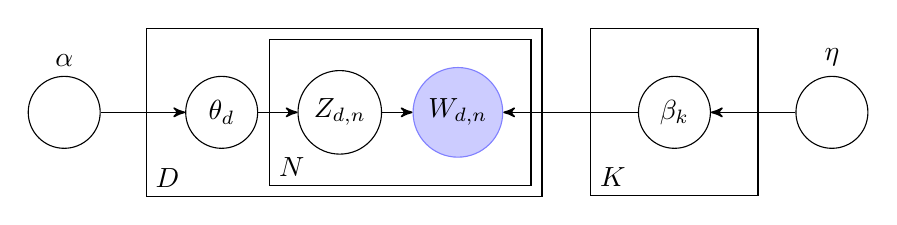
\begin{tikzpicture}
	    [
	      observed/.style={minimum size=15pt,circle,draw=blue!50,fill=blue!20},
	      unobserved/.style={minimum size=26pt,circle,draw},
	      post/.style={->,>=stealth',semithick},
	    ]
	
	    \node (w-j) [observed] at (0,0) {$W_{d,n}$};
	    \node (z-j) [unobserved] at (-1.5,0) {$Z_{d,n}$};
	    \node (theta) [unobserved] at (-3,0) {$\theta_d$};
	    \node (alpha-hyper) [unobserved, label=above:$\alpha$,left of=theta, node distance=2cm] {};
	    \node (beta-hyper) [unobserved] at (2.75,0) {$\beta_k$};
	    \node (eta-hyper) [unobserved, label=above:$\eta$, ,right of=beta-hyper, node distance=2cm] {};
	    
	    \path
	    (z-j) edge [post] (w-j)
	    (alpha-hyper) edge [post] (theta)
	    (theta) edge [post] (z-j)
	    (beta-hyper) edge [post] (w-j)
	    (eta-hyper) edge [post] (beta-hyper)
	    ;
	    
	    \node [draw,fit=(w-j) (theta), inner sep=14pt] (plate-context) {};
	    \node [above right] at (plate-context.south west) {$D$};
	    \node [draw,fit=(w-j) (z-j), inner sep=10pt] (plate-token) {};
	    \node [above right] at (plate-token.south west) {$N$};
	    \node [draw,fit=(beta-hyper) (beta-hyper), inner sep=17pt] (plate-context) {};
	    \node [above right] at (plate-context.south west) {$K$};
	  \end{tikzpicture}
  }
	\caption{Plate notation for \gls{lda}.}
	\label{fig:standard_lda}
\end{figure}

After training the \gls{lda} model, there are multiple possibilities for exploring the corpus using the posterior distributions of the hidden random variables.
One possibility is to visualize the posterior topics of the model, e.g., by sorting $\beta_k$ according to the highest probabilities.
It is also possible to visualize the documents by, e.g., sorting by the highest topic proportions in $\theta_d$.
Another possibility of exploration is finding similar documents by using a distribution distance function on the topic proportions $\theta_d$ between documents~\cite{blei2009topic}.

\subsection{Author-Topic \gls{lda} and Category-Topic \gls{lda}}
We model both of the metadata fields 'Author' and 'Category' similarly to the model presented by \citet{author_topic_2012}.
In this model, there are no document-topic distributions $\theta$.
Instead, each author and category has its own topic distribution.
This is based on the assumption that authors prefer to write about specific topics, and that categories of the articles were chosen based on the content of the finished article or that local newspapers have their own unique topic preferences.

Our topic models are \glspl{um}, meaning that topics are only word distributions and are chosen based on the data of the documents, rather than \glspl{dm} where topics are fitted to have an influence on both word distributions and other metadata.

\citet{author_topic_2012} describe the author-topic model where for each document $d$, they assign a vector of authors $a_d$ from a set of authors $A$, and for each word draw an author $x$ from this vector.
However, for our category-topic model and our own author-topic model, each document $d$ is associated with one category $c_d$ from a set of categories $C$ and one author $a_d$ from a set of authors $A$, rather than a vector.
This is due to our dataset never having more than one author or category for each document.
Unless otherwise stated, future mentions of the author-topic model are to our implementation of this model, rather than the model presented by \citet{author_topic_2012}.
The plate notation for our category and author \gls{lda} models can be seen in \autoref{fig:metadata_lda}.

\begin{figure*}[ht]
	\centering
	\begin{subfigure}{0.3\textwidth}
		\centering
		\resizebox{\textwidth}{!}{%
		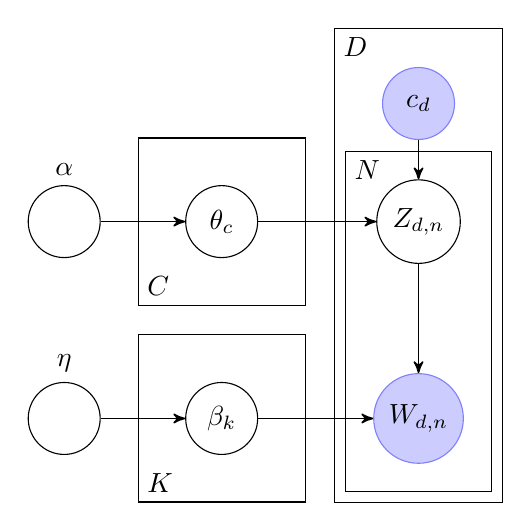
\begin{tikzpicture}
	[
	observed/.style={minimum size=26pt,circle,draw=blue!50,fill=blue!20},
	unobserved/.style={minimum size=26pt,circle,draw},
	post/.style={->,>=stealth',semithick},
	]
	
	\node (w-j) [observed] at (0,0) {$W_{d,n}$};
	\node (z-j) [unobserved, above of= w-j, node distance=2.5cm] {$Z_{d,n}$};
	\node (category_obs) [observed, above of= z-j, node distance=1.5cm] {$c_d$};
	\node (category_dist) [unobserved, left of=z-j, node distance=2.5cm] {$\theta_c$};
	\node (alpha-hyper) [unobserved, label=above:$\alpha$, left of=category_dist, node distance=2cm] {};
	\node (beta-hyper) [unobserved, left of = w-j, node distance=2.5cm] {$\beta_k$};
	\node (eta-hyper) [unobserved, label=above:$\eta$, left of=beta-hyper, node distance=2cm] {};
	
	\path
	(z-j) edge [post] (w-j)
	(alpha-hyper) edge [post] (category_dist)
	(category_obs) edge [post] (z-j)
	(category_dist) edge [post] (z-j)
	(beta-hyper) edge [post] (w-j)
	(eta-hyper) edge [post] (beta-hyper)
	;
	
	\node [draw,fit=(w-j) (category_obs), inner sep=14pt] (plate-context) {};
	\node [below right] at (plate-context.north west) {$D$};
	
	\node [draw,fit=(w-j) (z-j), inner sep=10pt] (plate-token) {};
	\node [below right] at (plate-token.north west) {$N$};
	
	\node [draw,fit=(beta-hyper) (beta-hyper), inner sep=17pt] (plate-context) {};
	\node [above right] at (plate-context.south west) {$K$};
	
	\node [draw,fit=(category_dist) (category_dist), inner sep=17pt] (plate-context) {};
	\node [above right] at (plate-context.south west) {$C$};
\end{tikzpicture}
		}
		\caption{Category \gls{lda}.}
		\label{fig:category_lda}
	\end{subfigure}
	\hspace{2em}
	\begin{subfigure}{0.3\textwidth}
		\centering
		\resizebox{\textwidth}{!}{%
			\begin{tikzpicture}
	[
	observed/.style={minimum size=26pt,circle,draw=blue!50,fill=blue!20},
	unobserved/.style={minimum size=26pt,circle,draw},
	post/.style={->,>=stealth',semithick},
	]
	
	\node (w-j) [observed] at (0,0) {$W_{d,n}$};
	\node (z-j) [unobserved, above of= w-j, node distance=2.5cm] {$Z_{d,n}$};
	\node (author_obs) [observed, above of= z-j, node distance=1.5cm] {$a_d$};
	\node (author_dist) [unobserved, left of=z-j, node distance=2.5cm] {$\theta_a$};
	\node (alpha-hyper) [unobserved, label=above:$\alpha$, left of=category_dist, node distance=2cm] {};
	\node (beta-hyper) [unobserved, left of = w-j, node distance=2.5cm] {$\beta_k$};
	\node (eta-hyper) [unobserved, label=above:$\eta$, left of=beta-hyper, node distance=2cm] {};
	
	\path
	(z-j) edge [post] (w-j)
	(alpha-hyper) edge [post] (author_dist)
	(author_obs) edge [post] (z-j)
	(author_dist) edge [post] (z-j)
	(beta-hyper) edge [post] (w-j)
	(eta-hyper) edge [post] (beta-hyper)
	;
	
	\node [draw,fit=(w-j) (author_obs), inner sep=14pt] (plate-context) {};
	\node [below right] at (plate-context.north west) {$D$};
	
	\node [draw,fit=(w-j) (z-j), inner sep=10pt] (plate-token) {};
	\node [below right] at (plate-token.north west) {$N$};
	
	\node [draw,fit=(beta-hyper) (beta-hyper), inner sep=17pt] (plate-context) {};
	\node [above right] at (plate-context.south west) {$K$};
	
	\node [draw,fit=(author_dist) (author_dist), inner sep=17pt] (plate-context) {};
	\node [above right] at (plate-context.south west) {$A$};
\end{tikzpicture}
		}
		\caption{Author \gls{lda}.}
		\label{fig:author_lda}
	\end{subfigure}
	\caption{Plate notation for the metadata \gls{lda} models.}
	\label{fig:metadata_lda}
\end{figure*}

\subsection{Pachinko Allocation}
In order to handle the hierarchical structure of the taxonomy metadata field, we use a hierarchical topic model, namely the \acrfull{pam} from \citet{li2006pachinko}.
Pachinko allocation generalizes \gls{lda}, making it possible to construct topic hierarchies based on any \gls{dag} structure.
\gls{pam} is a topic model focusing on finding topics of different abstraction levels and modeling the connections between these topics. 

Each node in the \gls{dag} structure represents a topic in the pachinko allocation model. 
However, unlike \gls{lda} where topics are distributions over words, in \gls{pam} topics are multinomial distributions over words and/or other topics further down the hierarchy of the \gls{dag} structure.
An example of the \gls{dag} structure used in this paper is shown in \autoref{fig:pachinko_dag}.

In this paper, we use a layered \gls{pam} meaning that the \gls{dag} structure is divided into layers, with every node in each layer fully connected to every node in the next layer of the hierarchy.
The first layer consists of only the root node, a topic which all documents are part of, and the bottom layer consists of leaf nodes, which are the only nodes to contain distributions over words, and they have no other topics in their distribution.

We replicate some layers in our \gls{dag} structure based on the structure from the taxonomy field within our dataset, having some nodes represent a topic based on a specific taxonomy.
To make the algorithm construct the topics to be based on our taxonomies, we introduce a novel locking mechanism for the Gibbs sampler which we use to run \gls{pam}.
This mechanism is discussed further in \autoref{subsec:mod_pachinko}.

We use a five-level pachinko tree structure, following the format presented by \citet{li2006pachinko}.
The first layer is the root layer.
The last layer is the word layer consisting of one node for each word in the vocabulary of our corpus.
The second and third layers will be constructed based on the entries of the first two positions in our taxonomy metadata, meaning there will be one node for each unique sub-taxonomy entry that is in the first or second position in the taxonomy sequence (e.g. "STEDER" and "Danmark", which is taken from "STEDER/Danmark/Aalborg", but not "Aalborg" since it is in the third position).
We only use the first two layers for this, as these are among the most informative, and because introducing even more layers would slow down the training exponentially, since the probability of all possible combinations of topics needs to be sampled for every word during training.
The fourth layer consists of $K = 90$ 'blank' topics, as with the other models we present in this paper.
This layer is added so that the model can construct its own topics based on the higher-level topics learned from our taxonomy metadata.
This \gls{dag} structure is visualized in \autoref{fig:pachinko_dag}.

The generative process for each document $d$ in \gls{pam} consists of the following steps, as described by \citet{li2006pachinko}:
\begin{enumerate}
	\item Sample $\theta_{t_1}^{(d)}, \theta_{t_2}^{(d)}, \dots, \theta_{t_s}^{(d)}$ from $g_1(\alpha_1), g_2(\alpha_2), \dots, \newline g_s(\alpha_s)$, where $\theta_{t_i}^{(d)}$ is a multinomial distribution of topic $t_i$ over its children.
	\item For each word $w \in d$,
	\begin{itemize}
		\item Sample a topic path $\mathbf{z}_w$ of length $L_w: < z_{w1}, z_{w2}, \dots, z_{wL_w} >$. $z_{w1}$ is always the root and $z_{w1}$ through $z_{wL_w}$ are topic nodes in $T$. $z_{wi}$ is a child of $z_{w(i-1)}$ and it is sampled according to the multinomial distribution $\theta_{z_{wL_w}}^{(d)}$.
		\item Sample word $w$ from $\theta_{z_{wL_w}}^{(d)}$.
	\end{itemize}
\end{enumerate}

$T = {t_1, t_2, \dots, t_s}$ os the set of topics in the \gls{pam}. 
Each topic $t_i$ is associated with a Dirichlet distribution $g_i(\alpha_i)$ based on a vector $\alpha_i$ which has the same dimention as the number of children in $t_i$.
While it is possible to use different $\alpha$ values for each topic, as shown here, we found through experimentation that using the same $\alpha$ value for all layers still provided good results.
An illustration of the plate notation for \gls{pam} can be found in \autoref{fig:pachinko}.

We use Gibbs sampling for performing inference.
For each word, a chain of topics is sampled by calculating the probability of all combinations of topics and making a weighted sample.
The probability of each topic combination is calculated using the joint probability of the topics, as presented in \autoref{eq:pachinko_gibbs}.

\begin{equation}\label{eq:pachinko_gibbs}
	\begin{split}
		P(Z_{w2} = t_a, Z_{w3} = t_b, Z_{w4} = t_c | \textbf{D}, z_{-w}, \alpha, \beta) \propto \\
		\frac{n_{1a}^d + \alpha_{1a}}{n_1^d + \sum_{a'} \alpha_{1a'}} \times
		\frac{n_{ab}^d + \alpha_{ab}}{n_a^d + \sum_{b'} \alpha_{ab'}}  \times 
		\frac{n_{bc}^d + \alpha_{bc}}{n_{b}^d + \sum_{c'} \alpha_{bc'}} \\ \times 
		\frac{n_{cw}^d + \beta_{w}}{n_{c} + \sum_{m} \beta_{m}} 
	\end{split}
\end{equation}
As in \citet{li2006pachinko}, $Z_{w2}$, $Z_{w3}$, $Z_{w4}$ are topic assignments for the three middle layers of topics in our 5-layer Pachinko model.
The root topic is not part of this equation since all words are part of it, so the probability does not need to be calculated.
$Z_{-w}$ is the word topic assignment, for all other words except the one that is being updated.
$n_x^d$ is the number of times topic $t_x$ occurs in document $d$ according to $Z_{-w}$. 
The $n_{xy}^d$ describes how many times topic $t_y$ is sampled from its parent $t_x$ within document $d$ according to $Z_{-w}$.
$n_x$ is the number of times topic $t_x$ occurs in the corpus according to $Z_{-w}$, and $n_{xw}$ is the number of times a word $w$ is in $t_x$ according to $Z_{-w}$.

\begin{figure}
	\centering
	\resizebox{0.8\columnwidth}{!}{%
	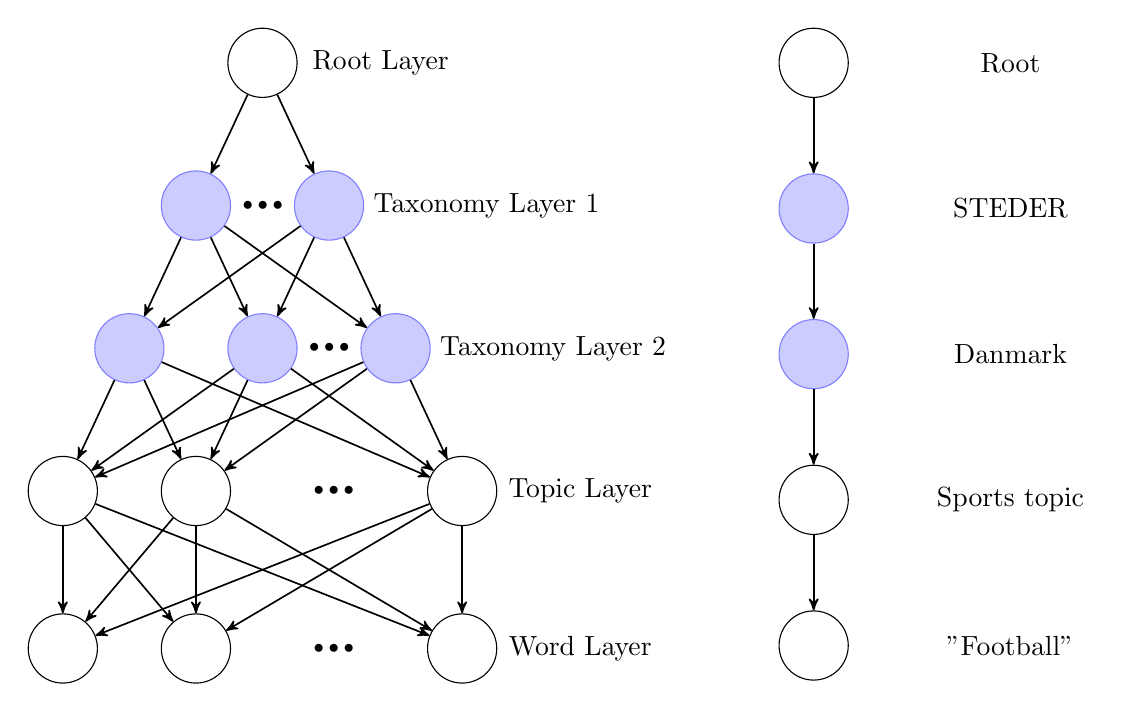
\begin{tikzpicture}
		[
		observed/.style={minimum size=25pt,circle,draw=blue!50,fill=blue!20},
		unobserved/.style={minimum size=25pt,circle,draw},
		post/.style={->,>=stealth',semithick},
		]
		% Layer 0
		\node (top) [unobserved] at (0,0) {};
		\node (topname) [right of = top, node distance=1.5cm] {Root Layer};
		
		% Layer 1
		\node (l11) [observed] at ([shift=({245:2 cm})]top) {};
		\node (l12) [observed] at ([shift=({295:2 cm})]top) {};
		\node (l1_dots) [right of = l11, node distance=0.85cm] {\scalebox{0.75}{$\bullet\bullet\bullet$}};
		\node (1name) [right of = l12, node distance=2cm] {Taxonomy Layer 1};
		
		% Layer 2
		\node (l21) [observed] at ([shift=({245:2 cm})]l11) {};
		\node (l22) [observed] at ([shift=({295:2 cm})]l11) {};
		\node (l23) [observed] at ([shift=({295:2 cm})]l12) {};
		\node (l2_dots) [right of = l22, node distance=0.85cm] {\scalebox{0.75}{$\bullet\bullet\bullet$}};
		\node (2name) [right of = l23, node distance=2cm] {Taxonomy Layer 2};
		
		% Layer 3
		\node (l31) [unobserved] at ([shift=({245:2 cm})]l21) {};
		\node (l32) [unobserved] at ([shift=({295:2 cm})]l21) {};
		\node (l33) [unobserved] at ([shift=({295:2 cm})]l23) {};
		\node (l2_dots) [right of = l32, node distance=1.75cm] {\scalebox{0.75}{$\bullet\bullet\bullet$}};
		\node (3name) [right of = l33, node distance=1.5cm] {Topic Layer};
		
		% Layer 4
		\node (l41) [unobserved] at ([shift=({270:2 cm})]l31) {};
		\node (l42) [unobserved] at ([shift=({270:2 cm})]l32) {};
		\node (l43) [unobserved] at ([shift=({270:2 cm})]l33) {};
		\node (l2_dots) [right of = l42, node distance=1.75cm] {\scalebox{0.75}{$\bullet\bullet\bullet$}};
		\node (4name) [right of = l43, node distance=1.5cm] {Word Layer};
		
		\path
		% Layer 0
		(top) edge [post] (l11)
		(top) edge [post] (l12)
		
		% Layer 1
		(l11) edge [post] (l21)
		(l11) edge [post] (l22)
		(l11) edge [post] (l23)
		(l12) edge [post] (l21)
		(l12) edge [post] (l22)
		(l12) edge [post] (l23)
		
		% Layer 2
		(l21) edge [post] (l31)
		(l21) edge [post] (l32)
		(l21) edge [post] (l33)
		(l22) edge [post] (l31)
		(l22) edge [post] (l32)
		(l22) edge [post] (l33)
		(l23) edge [post] (l31)
		(l23) edge [post] (l32)
		(l23) edge [post] (l33)
		
		% Layer 3
		(l31) edge [post] (l41)
		(l31) edge [post] (l42)
		(l31) edge [post] (l43)
		(l32) edge [post] (l41)
		(l32) edge [post] (l42)
		(l32) edge [post] (l43)
		(l33) edge [post] (l41)
		(l33) edge [post] (l42)
		(l33) edge [post] (l43)
		;
		
		
		\node (root) [unobserved, node distance=1.85cm] at (7,0) {};
		\node (rootname) [right of = root, node distance=2.5cm] {Root};
		
		\node (first) [observed, below of=root, node distance=1.85cm] {};
		\node (firstname) [right of = first, node distance=2.5cm] {STEDER};
		
		\node (second) [observed, below of=first, node distance=1.85cm] {};
		\node (secondname) [right of = second, node distance=2.5cm] {Danmark};
		
		\node (third) [unobserved, below of=second, node distance=1.85cm] {};
		\node (thirdname) [right of = third, node distance=2.5cm] {Sports topic};
		
		\node (fourth) [unobserved, below of=third, node distance=1.85cm] {};
		\node (fourthname) [right of = fourth, node distance=2.5cm] {"Football"};
		
		
		\path
		% Layer 0
		(root) edge [post] (first)
		(first) edge [post] (second)
		(second) edge [post] (third)
		(third) edge [post] (fourth)
		;
		
\end{tikzpicture}}
\end{figure}


\begin{figure}[h]
	\centering
	\resizebox{0.8\columnwidth}{!}{%
	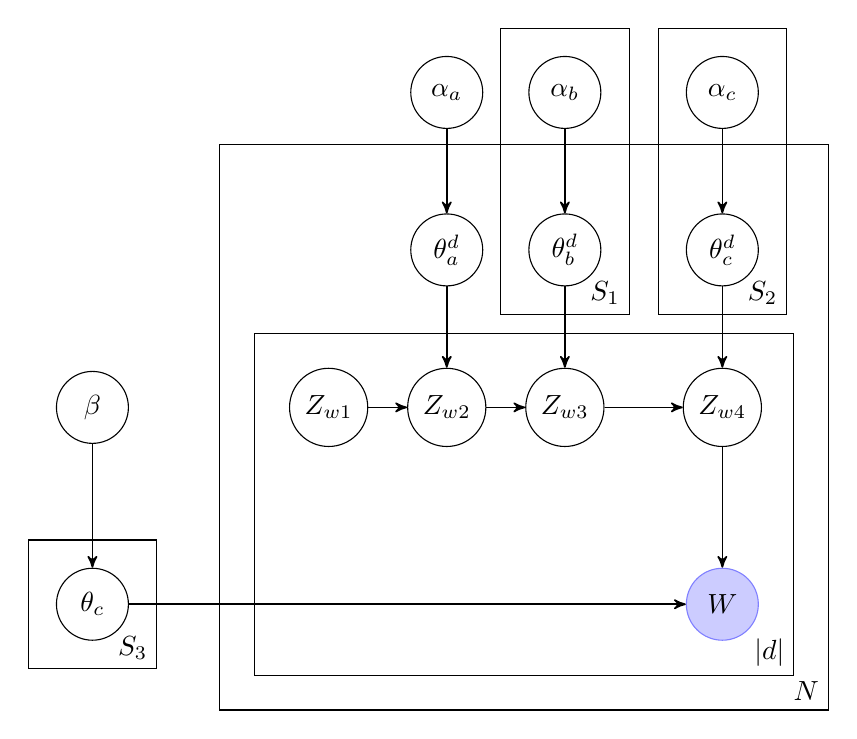
\begin{tikzpicture}
		[
		observed/.style={minimum size=26pt,circle,draw=blue!50,fill=blue!20},
		unobserved/.style={minimum size=26pt,circle,draw},
		post/.style={->,>=stealth',semithick},
		]
		
		\node (w-j) [observed] at (0,0) {$W$};
		\node (z-4) [unobserved, above of= w-j, node distance=2.5cm] {$Z_{w4}$};
		\node (z-3) [unobserved, left of= z-4, node distance=2cm] {$Z_{w3}$};
		\node (z-2) [unobserved, left of= z-3, node distance=1.5cm] {$Z_{w2}$};
		\node (z-1) [unobserved, left of= z-2, node distance=1.5cm] {$Z_{w1}$};
		
		\node (theta_a) [unobserved, above of= z-2, node distance=2cm] {$\theta_a^d$};
		\node (alpha_a) [unobserved, above of= theta_a , node distance=2cm] {$\alpha_a$};
		
		\node (theta_b) [unobserved, above of= z-3, node distance=2cm] {$\theta_b^d$};
		\node (alpha_b) [unobserved, above of= theta_b , node distance=2cm] {$\alpha_b$};
		
		\node (theta_c) [unobserved, above of= z-4, node distance=2cm] {$\theta_c^d$};
		\node (alpha_c) [unobserved, above of= theta_c , node distance=2cm] {$\alpha_c$};
		
		\node (theta_s2) [unobserved, left of=w-j , node distance=8cm] {$\theta_c$};
		\node (beta) [unobserved, above of=theta_s2 , node distance=2.5cm] {$\beta$};
		
		\path
		(z-4) edge [post] (w-j)
		(z-3) edge [post] (z-4)
		(z-2) edge [post] (z-3)
		(z-1) edge [post] (z-2)
		
		(theta_a) edge [post] (z-2)
		(alpha_a) edge [post] (theta_a)
		
		(theta_b) edge [post] (z-3)
		(alpha_b) edge [post] (theta_b)
		
		(theta_c) edge [post] (z-4)
		(alpha_c) edge [post] (theta_c)
		
		(theta_s2) edge [post] (w-j)
		(beta) edge [post] (theta_s2)
		;
		
		\node [draw,fit=(w-j) (theta_a) (z-1), inner sep=25pt] (plate-context) {};
		\node [above left] at (plate-context.south east) {$N$};
		
		\node [draw,fit=(w-j) (z-1), inner sep=12.5pt] (plate-token) {};
		\node [above left] at (plate-token.south east) {$|d|$};
		
		\node [draw,fit=(theta_s2), inner sep=10pt] (plate-token) {};
		\node [above left] at (plate-token.south east) {$S_3$};
		
		\node [draw,fit=(theta_c) (alpha_c), inner sep=10pt] (plate-token) {};
		\node [above left] at (plate-token.south east) {$S_2$};
		
		\node [draw,fit=(theta_b) (alpha_b), inner sep=10pt] (plate-token) {};
		\node [above left] at (plate-token.south east) {$S_1$};
		
	\end{tikzpicture}}
	\caption{Plate notation for the five-level \gls{pam}.}
	\label{fig:pachinko}
\end{figure}
\vejleder[inline]{a,b,c ~ $t_i$ in Figure 5}

\subsubsection{Modification to Pachinko Allocation}\label{subsec:mod_pachinko}
Without modification, \gls{pam} will find topics with the same structure as our taxonomy, but the topics will not actually be based on the taxonomy.
However, only $25\%$ of the documents in our dataset have an observed taxonomy.
To account for this, we lock taxonomy for the words in the observed documents to be in the corresponding topics within the pachinko \gls{dag} instead of continuously sampling them using Gibbs sampling.
This creates a constant context for the taxonomy topics, which the documents with unobserved taxonomies will be fitted around.

Some of the observed documents have multiple taxonomies.
For these documents, one of the taxonomies is chosen randomly for each word in the document.


%
%\input{sections/method/preprocessing}
%\input{sections/method/method.tex}
%\input{sections/method/query_handling.tex}

%\section{Dataset}
Nordjyske is a Danish news agency that maintains multiple newspapers, radios and other news sources throughout north Jutland, a region in Denmark.
They store their news articles in a non-public database, where each article contains multiple meta-data fields which describes some aspect of the data eg. author.
The dataset is from 2017 to 2019 and contains 139261 articles which uses a vocabulary of 69192 unique words.
One of the metadata fields is the Category field, which both describes where the article is supposed to be located(within a newspaper) and also which subject the article is about.
These meta-data are very interesting in that they detail the data in certain ways which might be useful in some way.

In the following section, we describe each of the meta-data fields which are analysed.

\subsection{Author}
This field mentions the author, who have written the article.
Each article only has a single author, so we do not account for multiple authors in this paper.
This field is fully observed within the dataset, which means that every article has an author.
There are $227$ different authors within the dataset and they are almost evenly distributed in the number of articles they have written.

\subsection{Category}
The category field describes a variety of different aspects. 
This field is fully observed within the dataset and there are $58$ different categories.
A proportion of the articles contains which specific newspaper, they belong to, eg. Aalborg-Newspaper.
Another proportion of the category fields describes the overall theme, such as Culture and Sports-newspaper.

\subsection{Taxonomy}
The taxonomy field describes a hierarchical structure of the topical or geographical subject of the articles.
This field is only partially observed within the dataset, which means that roughly $50\%$ of the articles contain this field.
We observe a general pattern when traversing this field which is:
\begin{itemize}
	\item Places/Country/Region/Town
	\item Topics/Sub-Topic/Subsub-topic
\end{itemize}
Examples of this field are:
\begin{itemize}
	\item PLACES/Danmark/Nordjylland/Aalborg/Lillevorde
	\item TOPICS/Religion/Christianity
\end{itemize}
%%\input{sections/Pipeline.tex}
\section{Evaluation}\label{sec:experiment}
In this section, we evaluate the topic models previously defined.
We also define the evaluation metrics and how hyperparameters for the models were chosen.
Lastly, the results of the evaluations are displayed.

\subsection{Models}\label{sec:experiment_models}
A list of different topic models is evaluated each using different metadata from the dataset.
The main difference between the models is how they draw a specific topic for a word.
As detailed in \autoref{sec:plate_notation} the main models used in this experiment are:
\begin{description}
	\item[\Acrlong{lda}] Standard \gls{lda} which uses document-topic distributions.
	\item[Author-Topic Model]\cite{author_topic_2012} An \gls{lda} based model, which uses author-topic distributions.
	\item[Category-Topic Model] An \gls{lda} based model which uses category-topic distributions.
	\item[Taxonomy-Topic Model] A \acrlong{pam} which uses hierarchical taxonomy information.
\end{description}

\subsection{Evaluation Metrics}\label{sec:experiment_metrics}
\vejleder[inline]{fix commas in this section}
All models previously mentioned are evaluated using the following evaluation metrics.

The main metric used in this experiment is the topic coherence metric.
This metric indicates how semantically similar the top words within each topic are and is an indication of the topic quality within a model~\cite{topic_coherence_2015}.
There are different methods for calculating topic coherence, but we will be using $C_v$ coherence.
$C_v$ is calculated using the following steps, as presented by~\citet{Syed2017coherence}:
\begin{enumerate}
	\item Topic-word segmentation into word set pairs
	\item Word and word pair probability calculation
	\item Word set confirmation measure
	\item Aggregation of confirmation measures
\end{enumerate}
The intuition is to calculate the degree of semantic similarity between highly probable words in a topic.
This intuition, and each step, is explained further in Appendix \autoref{app:topic_coherence}.

The second metric used in the experiment is perplexity.
Perplexity is used as a metric to show how well a model can predict new test samples $w_d$.
But because perplexity is not specific to topic models and by itself does not give an indication of how coherent topics are, it is used as a secondary evaluation~\cite{tea_leaves}.
To calculate perplexity, we first need to compute the log-likelihood of $w_d$, which is done in:
\begin{equation}\label{eq:likelihood}
	\mathcal{L}(w_d) = \log p(w_d|\Phi) = \sum_{d} \log p(w_d|\Phi)
\end{equation}
\noindent where $\Phi$ is the topic-word matrix.
The perplexity measure is then calculated as follows:
\begin{equation}
	\emph{Perplexity}(w_d) = exp \{-\frac{\mathcal{L}(w_d)}{W}\}
\end{equation}
\noindent where W is the number of words \cite{de2008evaluating}.

The second metric used in the experiment is topic difference.
Topic difference is another metric that is used to check the quality of the topic model.
It is based on the assumption that a good topic model will have little overlap between topics.
It is therefore not the best measure of the final quality of a topic model but a low topic difference will indicate potential problems with a model.
\begin{equation}
	\emph{TopicDifference} = \frac{1}{K \cdot K} \sum_{i=1}^{K} \sum_{j=1}^{K} JS(\beta_{i},\beta_{j})
\end{equation}
\noindent where $JS$ is Jensen-Shannon distance, $K$ is the number of topics, and $\beta_{k}$ is the topic-word distribution for topic $k$.
If the total sum is not averaged, it can also be used to indicate the convergence of the model.

\subsection{Grid Search}\label{sec:experiment_gridsearch}
To find the optimal hyperparameter values for the models, we run a grid search.
To find the best performing model we test different values of $K$, $\alpha$, and $\eta$ in a grid search.
Specifically, we run two rounds of grid search.
In the first round, the number of topics $K$ we test are the values of $K_1$, as seen in \autoref{tab:gridsearch}, with randomly chosen $\alpha$ and $\eta$ values for each $K$ value.
This creates much fewer runs of the grid search to start with and eliminates hyperparameter values that give worse models.
In the second round, the number of topics $K$ we test are the values of $K_2$ with all combinations of $\alpha$ and $\eta$ except for those with values of $0.001$, since these models gave much worse scores.
The hyperparameter values used are shown in \autoref{tab:gridsearch}.

We only run the grid search on the standard \gls{lda} model, with the assumption that the number of topics that perform well for this model also performs well for the metadata models when the same dataset is used.
To evaluate the \gls{lda} models, we measure the topic coherence of a model after training it on the dataset for 50 epochs, and the hyperparameters of the model with the highest score are then used for the models in the rest of the experiment.

Based on the topic coherence of the model, we choose $K = 90$, $\alpha = 0.01$, and $\eta = 0.1$ as the hyperparameters for all models in the experiment.

\begin{table}[t]
	\centering
	\caption{Tested hyperparameter values for the grid search. $K_2$ are the $K$ values used for the grid search in conjunction with the bolded values in $\alpha$ and $\eta$.}
	\begin{tabular}{c|c}
		Parameter & Tested Values\\
		\midrule
		$K_1$ & 10, 20, 30, $\dots$, 100, 150\\
		$K_2$ & 50, 60 70, 80, 90, 100\\
		$\alpha$ & \textbf{0.1}, \textbf{0.01}, 0.001\\
		$\eta$ & \textbf{0.1}, \textbf{0.01}, 0.001\\
	\end{tabular}
	\label{tab:gridsearch}
\end{table}


\subsection{Results}\label{sec:results}

\begin{table}[h]
	\centering
	\caption{Results.}
	\begin{tabular}{l|c|c}
		Topic Model & \makecell{Topic \\ Coherence} & \makecell{Topic \\ Difference} \\
		\midrule
		\Acrlong{lda} & 0.520 & 0.575 \\
		Author-Topic Model & 0.335 & 0.615 \\
		Category-Topic Model & 0.370 & 0.560 \\
		Taxonomy-Topic Model & \textbf{0.660} & \textbf{0.709} \\
	\end{tabular}
	\label{tab:metric_results}
\end{table}

From \autoref{tab:metric_results}, we can see that the Author and Category-Topic models are performing the worst, whereas the Taxonomy-Topic model is outperforming all other models.
However, the elapsed time of the taxonomy-topic model is worse than the standard \gls{lda}.
It takes about $6$-$8$ hours to compute $50$ epochs for the \gls{lda} model, depending on the CPU. 
The taxonomy-topic model running a $5$ layered \gls{pam} took ${\sim}132$ hours before completing the $50$ epochs.
Analysis of the topics in the trained models is given in \autoref{sec:discussion}.
Extended analysis and other models are investigated in Appendix \autoref{subsec:app_exten_models} and \autoref{app:cat_auth_pachinko}.


%% - Body(50 \%)
%%	- Results 
%
%%	- Discussion
%%		- Main results
%%		- Other results
%%		- Error sources
\section{Discussion}\label{sec:discussion}
In this section, we investigate the different models to see how each meta-information field impacts the resulting topics.
Firstly, we want to investigate the top words within each model.
We have taken a random article from the dataset and visualized how the topics differ between the models. 
Before investigating the article below, we define a specific color scheme for each model.

In the article, we have highlighted the highest probable words within the three most occurring topics in the article.
The article is about agriculture and how farmers are letting their cows out onto grass fields in September. 
It also mentions a few different farms in the Northern part of Jutland and describes these in various ways.

The way we can compare these models, is by taking the top 200 words for each topic-word distribution within each model and marking them in the article below.
Since the Author and Category models do not have a document-topic distribution we can not look at the specific document, but instead we have marked the words from the given category- and author-topic distribution within the document, to see what the difference in topics are.
We are looking at the top 3 topics within each model for the specific document.

\begin{table}[h]
	\centering
	\caption{Color scheme for each model.}
	\begin{tabular}{l|c}
		Topic Model & Color \\
		\midrule
		\Acrlong{lda} & \thiscolor{Goldenrod} \vspace*{2mm} \\
		Author-Topic Model & \thiscolor{Aquamarine} \vspace*{2mm} \\
		Category-Topic Model & \thiscolor{LimeGreen} \vspace*{2mm} \\
		Word appearing in multiple models & \thiscolor{Peach} \vspace*{2mm}  \\
	\end{tabular}
	\label{tab:disc_color}
\end{table}

\emph{
Kig på grise, køer og kyllinger10 \colorbox{Peach}{nordjyske} bedrifter åbner \colorbox{LimeGreen}{søndag} for stalddørene Landbruget åbner \colorbox{LimeGreen}{søndag} 16. \colorbox{Peach}{september} ladeporte og stalddøre for offentligheden. 52 danske bedrifter er med i årets ”Åbent landbrug”. I det \colorbox{Peach}{nordjyske} kan man kigge forbi på 10 \colorbox{Peach}{forskellige} landbrug. Blandt de \colorbox{Peach}{nordjyske} deltagere er der \colorbox{Peach}{mulighed} for at få indsigt i både kvæg- og svinebedrifter, \colorbox{Peach}{ligesom} en producent af slagtekyllinger \colorbox{Aquamarine}{byder} velkommen. Sidstnævnte kan opleves hos Rokkedahl i Farstrup. De er tre familier med i alt \colorbox{Peach}{seks} børn, der sammen driver Rokkedahl Landbrug med slagtekyllinger og planteproduktion \colorbox{Peach}{samt} Rokkedahl Energi, som laver energioptimering. Herudover har de \colorbox{Goldenrod}{eget} slagteri, hvor ca. 35 af deres i alt 65 \colorbox{Peach}{medarbejdere} arbejder. Familien Rokkedahl har \colorbox{Peach}{arbejdet} med kyllinger siden 1963 og er tredje generation. I staldene og i de omkringliggende folde har de både fritgående og økologiske slagtekyllinger. Velfærdskyllingerne går i flokke og har adgang til store folde. På årsbasis opdrætter Rokkedahl \colorbox{Peach}{otte} \colorbox{Peach}{millioner} kyllinger som enten slagtes på deres \colorbox{Goldenrod}{eget} slagteri eller sælges til eksterne slagterier. På de 1350 \colorbox{Goldenrod}{hektar} har de hvede, byg raps, havre, rug, ærter og hestebønner. Det anvendes primært til foder til velfærdskyllingerne. De dyrker \colorbox{Peach}{jorden} primært økologisk og anvender halmen til opvarmning af staldene. De har varmevekslere på alle stalde for at minimere varmeforbruget og ammoniakudledningen til omgivelserne. Britt og Klaus Kristiansen på Solbakken Agri ved Aabybro er \colorbox{Peach}{klar} til vise en stor, \colorbox{Peach}{dansk} mælkeproduktion frem. Familien tæller også de fire børn, Maria på 18 år, Daniel på 16 år, Kamilla og Laura på 13 år, og de er sjette generation på gården, som de overtog i 2013. Solbakken har 600 økologiske malkekøer, som tilsammen \colorbox{Peach}{giver} 17.000 liter mælk om dagen. Den bliver hentet og kørt til et af Arlas mejerier, hvor den bliver anvendt til økologiske mejeriprodukter. 575 \colorbox{Goldenrod}{hektar} \colorbox{Peach}{land} tilhører gården, og her producerer \colorbox{Goldenrod}{familien} foder til deres \colorbox{Peach}{dyr} \colorbox{Peach}{samt} andre fødevarer.  I Himmerland kan man besøge Sanne og Ole Mathiasen, der driver Nørregaard på Braulstrupvej 9 i Suldrup. Her kan man se søer, smågrise og slagtesvin i staldene og \colorbox{Aquamarine}{høre} om \colorbox{Goldenrod}{produktion} af velfærdsgrise, se maskinerne, få smagsprøver fra Danish Crown og på \colorbox{Peach}{lokale} fødevarer, og \colorbox{Aquamarine}{høre} om biavl. For \colorbox{Aquamarine}{børnene} er der \colorbox{LimeGreen}{leg} i korncontainer og halm, pedaltraktorbane og ponytrækketure. Der er kaffe og kagebord. Åbent \colorbox{Goldenrod}{landbrug} foregår \colorbox{LimeGreen}{søndag} fra \colorbox{LimeGreen}{klokken} 10 til 16. Det er gratis at deltage. Sidste år deltog 96.000 \colorbox{LimeGreen}{danskere} i åbent landbrug.
}

Overall, we see that there is a large amount of overlap between the models, which is interesting since the models use different meta-information to create the various topic distributions.
This indicates that the models share many of the top words, while also indicating a slight deviation between the models due to the meta-information.
The \gls{lda} model shows words like "landbrug" (agriculture) and "produktion" (production), which is what the article is mostly about.
This behavior is to be expected since the performance of \gls{lda} has been explored and evaluated before. 
Author-topic specific words are not very present and are only showing three unique words: "byder", "hører", and "børnene".
This indicates that the Author-topic model has trouble generalizing what the author of this article (Peter Tordrup Larsen) is writing about, possibly because he has written $5002$ articles in our dataset.
Another aspect of the Author-Topic model is that the authors writing these articles most likely do not write about just one subject, which explains why there is only three less important words marked here. 
The Category-topic model only shows four unique words: "søndag", "leg", "klokken", and "danskere".
These words are also very abstract and can be used in many different scenarios.

An interesting part of this analysis is the words appearing in multiple models.
Some of the words within this category are: "arbejdet", "jorden", "dyr", and "nordjyske".
These words summarize the text pretty well, but it is also hard to summarize this text since it covers a wide variety of specific topics.
Combining the results of these models might yield better topic models, but we can not conclude that based on only one article.
There is also the possibility that choosing another random article would give completely different numbers of marked words per model, because this highly depends on the article's author and category.


\subsection{Author-topic model}\label{sec:discussion_author_topic}
Some interesting observations can also be made specifically in the author-topic model.
One observation that is possible, is looking at the similarity of authors.
In this model, the author-topic distribution defines the probabilities of topics being written by a specific author.
Then, just as \citet{author_topic_2012}, the similarity of authors can be found by calculating the symmetric Kullback-Leibler divergence:

\begin{equation}
	sKL(i,j) = \sum_{t=1}^{T}\left[\theta_{it}\, log \frac{\theta_{it}}{\theta_{jt}} + \theta_{jt}\, log \frac{\theta_{jt}}{\theta_{it}}\right]
\end{equation}
\noindent where $\theta_{it}$ is the probability of author $i$ having written about topic $t$, and the same for $\theta_{jt}$ with author $j$.

In the context of using these similarities to assist Nordjyske, knowing how similar authors are gives the opportunity to recommend new authors to readers, while the articles are about similar topics.
In \autoref{tab:author_similarity} the top 10 author pairs, based on this similarity measure, are shown.
A smaller KL value means the authors are more similar.
The number in parenthesis next to each author is the number of articles they have written in our dataset.

\begin{table}[h]
	\centering
	\caption{Top 10 author pairs based on the symmetric KL divergence between authors.}
	\begin{tabular}{r|c}
		Author pair & KL \\
		\midrule
		Lars Termansen (328) \& Mikkel Færgemann Viken (91) & 1.50 \\
		Morten Nis Klenø (17) \& Anne Helene Thomsen (606) & 1.72 \\
		Lars Termansen (328) \& Lars Christensen (1293) & 2.43 \\
		Esben Heine Pedersen (1689) \& Caspar Birk (71) & 2.47 \\
		Lars Christensen (1293) \& Poul Christoffersen (65) & 2.53 \\
		Lone Beck (92) \& Max Melgaard (587) & 2.74 \\
		HANNE Lindblad Jensen (27) \& Peter Tordrup Larsen (5002) & 2.94 \\
		Søren Kjær (95) \& Carl Chr. Madsen (785) & 2.98 \\
		Heidi Majgaard B. Pedersen (244) \& Lisbeth Helleskov (361) & 3.05 \\
		Lars Termansen (328) \& Morten Lind (413) & 3.16 \\
		\midrule
		Maximum & 34.51 \\
		Median & 24.20 \\
	\end{tabular}
	\label{tab:author_similarity}
\end{table}

In general for these pairs, there does not seem to be a correlation between a high similarity and the categories of the articles they have written.
While one author in a pair might have written for the sports category (Sport-avis) the other author might not have written for this category at all.
This can also be seen for categories that cover geographic locations, where one author might have written for Aalborg (Aalborg-avis) and the other author can have written for Thisted (Thisted-avis).

When looking at a sample of documents for the most similar author pair (Lars Termansen \& Mikkel Færgemann Viken), it is seen that they both write a mix of regular news and sports articles.
The reason why they become this similar, might be that the ratio between news and sports news for both authors is similar, and possibly also because of the types of news they write about.
Another interesting observation is that, for the second most similar author pair (Morten Nis Klenø \& Anne Helene Thomsen) the difference in the number of articles written is significant.
Here Morten Nis Klenø has written just 17 articles while Anne Helene Thomsen has written 606 articles.
This suggests that some part of why these authors' similarity is high, simply dependents on the types of news the authors have written, no matter the amount.

It is also worth noting that while authors that write scientific papers usually write in just a few subject areas, the scientific area they work in, this is not the case for news article authors.
In our dataset, this can be seen in the fact that the authors have written for 7.86 categories on average, with 7 categories as the median.
This can make it more difficult for the author-topic model to find patterns in what the authors write about, especially since each category can cover multiple topics.

A selection of authors from the dataset and the top words from their most probable topics, can be seen in \autoref{tab:author_top_words}.

\begin{table*}[h]
	\centering
	\caption{Selection of authors and the top 10 words from their most probable topic.}
	\begin{tabular}{c|c|c|c|c|c|c}
		\toprule
		Birgitte Bové & Kirsten Østergaard & Pauline Bülow & Karen Marie Foldbjerg & Claus T. Kræmmergård & Hanne Lindblad Jensen & Ole Jensen \\
		\midrule
		Topic 41 & Topic 50 & Topic 3 & Topic 13 & Topic 88 & Topic 2 & Topic 50 \\
		\midrule
		\makecell{millioner \\ eu \\ hans \\ større \\ bedre \\ formand \\ kr \\ nordjyske \\ taget \\ skriver} & \makecell{du \\ thisted \\ unge \\ mig \\ børn \\ procent \\ hans \\ hver \\ penge \\ hjørring} & \makecell{procent \\ bag \\ rigtig \\ lave \\ dansk \\ formand \\ gode \\ klar \\ svært \\ plads} & \makecell{du \\ sine \\ formand \\ seneste \\ jensen \\ hvert \\ nyt \\ hvordan \\ finde \\ kommunen} & \makecell{du \\ procent \\ unge \\ børn \\ arige \\ hans \\ dansk \\ mig \\ thisted \\ mener} & \makecell{du \\ thisted \\ procent \\ mig \\ børn \\ hans \\ unge \\ dansk \\ mener \\ a} & \makecell{du \\ thisted \\ unge \\ mig \\ børn \\ procent \\ hans \\ hver \\ penge \\ hjørring} \\
		\bottomrule
	\end{tabular}
	\label{tab:author_top_words}
\end{table*}

As can be seen through this analysis, this knowledge about authors and their topic probabilities can be useful for making better news recommendation systems, but it will be limited since news authors usually write about multiple subjects.

%
%
%% - Conclusion (5 \%)
%%	- (Possible) Future work
\section{Conclusion}\label{sec:conclusion}
In this paper, we explore possibilities for incorporating metadata into existing topic models, such as \gls{lda} and \gls{pam}.
We evaluate these models based on three different metadata: Author, Category, and Taxonomy, each of which represents the data in a different way.

From the topic coherence results, shown in \autoref{tab:metric_results}, the \gls{pam} model using the Taxonomy metadata gets the best results.
The Author and Category models based on \gls{lda} are the worst-performing, where the topic coherence is much lower than the other models.

We want to answer the problem statement, which we stated in \autoref{sec:introduction}:


\begin{itemize}
	\item \textit{How does including metadata within the \gls{lda} model impact the resulting topics?}
	\item \textit{What possible problems can these models help alleviate at Nordjyske?}
	\begin{itemize}
		\item \textit{More specifically, how can these models improve recommendation?}
	\end{itemize}
\end{itemize}

We incorporate metadata into our topic models in multiple ways.
The \gls{lda} model is used as a baseline, which indicates whether incorporating metadata can improve the topic quality of our topic models.
Based on the results of Author-Topic and Category-Topic, we see that only using the metadata for topic assignment within \gls{lda} can hurt the topic quality.
Other studies have shown that only using the metadata for topic assignment can improve the performance.
This might be due to the particularities of the dataset, such as authors not usually writing about the same subject within the news environment.  


We use the \gls{pam} to incorporate a hierarchically structured metadata called Taxonomy, where we use a novel locking mechanism to lock the observed metadata's topics into place.
Using this model and technique, we can get better topic quality and words within \gls{pam} compared to the \gls{lda}.
However, the run time of the algorithm is quite slow compared to the \gls{lda}.
All models ran for 50 epochs, but \gls{pam} had a runtime of 130 hours, compared to \gls{lda} which had a runtime of 8 hours.

Topic modeling can be used to alleviate many problems at Nordjyske, such as recommendations.
We can use the topic distributions from our models to compare articles based on their similarity in topics.
For example, the author-topic model's topic distribution can be used to recommend similar authors, while in the topic distributions of the taxonomy model, there is the possibility of looking at topics from different layers.
This information can be used in a content-based filtering approach to recommend similar articles.
We suggest using this topic information to enrich the recommendation process at Nordjyske. 

Due to the promising results provided by the modified pachinko model, investigating this model further might be beneficial to incorporating metadata into topic models.
However, testing these models on multiple datasets needs to be accounted for since the generalizability of these models is not explored within this paper.
Using word embedding to further improve the performance of models can also be viewed as a possible next step for this project since a wide number of papers are using this technique to improve topic modeling\cite{MetaLDA2017}\cite{dieng2020topic}.

It would also be interesting to see how we could incorporate these models into an existing IT infrastructure at Nordjyske.
The next step in that process would be to investigate which part of their infrastructure could benefit from the use of topic modeling, whether it is for recommendation or automatic tagging of articles. 
We have written about a few potential use cases of our project in Section \ref{sec:appendix_applications} in the Appendix. 

%
%\input{sections/Acknowledgements}

% - References (10 \%)
% 	- Acknowledgments
%	- Bibliography
\bibliography{paper}

%Appendixes, if needed, appear before the acknowledgment.
\appendix
\subsubsection{Metadata labels}\label{sec:appendix_meta_data}
Here are the 58 different categories, which make up all the category labels present within the dataset.

\begin{table*}[h]
	\centering
	\begin{tabular}{l|c|l|c|l|c|l|c}
		Category & Number & Category & Number & Category & Number & Category & Number \\
 		\toprule
		Udland-avis & 8855 & 26. Frederik & 484 & INFOMAKER PRINT & 5 & Thisted sport & 698\\
		Kram & 244 & Feature & 188 & Thisted-net & 3 & WEEKEND & 1493\\
		Navne & 3749 & Morsø-avis & 5959 & DF Licitation Diverse & 4 & Erhverv-avis & 7356\\
		Brønderslev-net & 3857 & Aalborg-avis & 5544 & Oplandsavisen & 6 & Biler & 13\\
		Fælles & 20204 & Mariagerfjord-avis & 7241 & Morsø Sport & 2350 & Sport-net & 3\\
		Bo Godt & 1447 & Erhvervsnavne & 39 & Debat & 10075 & Frieord & 1341\\
		RB & 3 & Hanbo-bladet & 2 & Lokalavisen & 1 & Indsigt & 984\\
		Samfund & 9 & Morsø Debat & 1375 & Sport-avis & 10941 & Kultur & 3012 \\
		53. Frederik & 203 & DF Søfart & 32 & Bagside & 1933 & Morsø-net & 1 \\
		Frederikshavn-avis & 4325 & Nordjyske Biler & 1400 & Østvendsyssel Avis & 4 & Aalborg:nu & 73\\
		Perspektiv & 613 & Brønderslev-avis & 3857 & Rebild-avis & 4415 & Brugermappe & 1\\
		Thisted-avis & 11473 & DF Motor Biler & 3 & Nyhedsmotoren-net & 3 & Morsø Ugeavis & 27\\
		Jammerbugt-avis & 3791 & MitLiv & 1519 & Newspack & 35 & DF Licitation Byggeri & 14\\
		Mariagerfjord-net & 1 & Hjørring-avis & 4235 & Friii & 2333 & Vesthimmerland-avis & 5131\\
		Plus Publicering & 3 & Nordjyske Plus & 6 & & & & \\
		\bottomrule
	\end{tabular}
	\caption{Amount of documents with each category within the Nordjyske dataset from 2017 to 2019.}
	\label{tab:category_table}
\end{table*}

%\input{sections/appendix/query_expansion.tex}
%\input{sections/appendix/variational_inference.tex}
%\input{sections/appendix/problems.tex}
%\input{sections/appendix/search_result.tex}
%\input{sections/appendix/perplexity_granularity.tex}
%\input{sections/appendix/word_count_distributions.tex}
%\input{sections/appendix/topic_documents.tex}

% Examples of tables and figure
%\input{examples.tex}

%\section{Unused Sections}
%\input{unusedSections/KnowledgeGraph.tex}
\end{document}
